\documentclass[12pt]{article}
\usepackage[margin=2.5cm]{geometry}
\usepackage{titling}
\usepackage{enumerate}
\usepackage{graphicx}
\usepackage{mdframed}
\usepackage{listings}
\usepackage{xcolor}

\definecolor{codegreen}{rgb}{0,0.6,0}
\definecolor{codegray}{rgb}{0.5,0.5,0.5}
\definecolor{codepurple}{rgb}{0.58,0,0.82}
\definecolor{backcolour}{rgb}{0.95,0.95,0.92}

\lstdefinestyle{mystyle}{
    backgroundcolor=\color{backcolour},
    commentstyle=\color{codegreen},
    keywordstyle=\color{magenta},
    numberstyle=\tiny\color{codegray},
    stringstyle=\color{codepurple},
    basicstyle=\ttfamily\footnotesize,
    breakatwhitespace=false,
    breaklines=true,
    captionpos=b,
    keepspaces=true,
    numbers=left,
    numbersep=5pt,
    showspaces=false,
    showstringspaces=false,
    showtabs=false,
    tabsize=1
}

\lstset{style=mystyle}

\predate{}
\postdate{}

\begin{document}
\title{Lab 3 Task 4 Solution}
\date{}
\maketitle


\section*{4) Plan a Player class and 3 subclasses}
\begin{enumerate}[1.]
    \item Get out some paper and write down the four class names \textit{Player},
    \textit{RandomPlayer},\\ \textit{StrategicPlayer}, and \textit{UserPlayer} with lots
    of space below each in which to describe their data and their methods.

    \bigskip

    \begin{figure}[h]
        \centering
        \begin{tabular}{|p{3.25cm}|}
            \hline
            \textbf{Player}\\
            \hline
            \\
            \\
            \\
            \hline
            \\
            \\
            \\
            \hline
        \end{tabular}
        \begin{tabular}{|p{3.25cm}|}
            \hline
            \textbf{RandomPlayer}\\
            \hline
            \\
            \\
            \\
            \hline
            \\
            \\
            \\
            \hline
        \end{tabular}
        \begin{tabular}{|p{3.25cm}|}
            \hline
            \textbf{StrategicPlayer}\\
            \hline
            \\
            \\
            \\
            \hline
            \\
            \\
            \\
            \hline
        \end{tabular}
        \begin{tabular}{|p{3.25cm}|}
            \hline
            \textbf{UserPlayer}\\
            \hline
            \\
            \\
            \\
            \hline
            \\
            \\
            \\
            \hline
        \end{tabular}
    \end{figure}

    \item You are going to make a simple diagram like Figure ~\ref{fig:uml}.

    \begin{figure}
        \begin{center}
        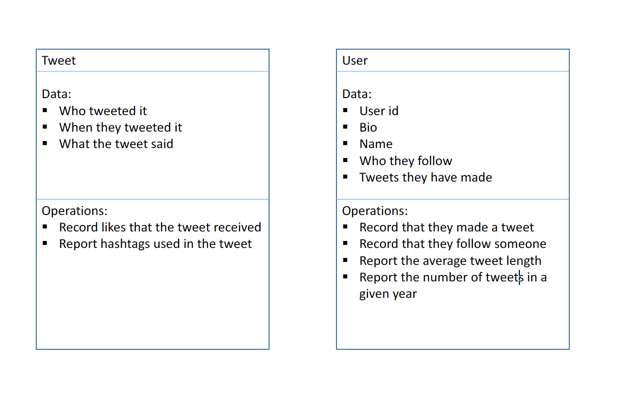
\includegraphics[width=0.8\linewidth]{../../images/lab_3/uml.png}
        \end{center}
        \caption{Design for twitter example}
        \label{fig:uml}
    \end{figure}

    \item You already identified which methods are needed based on your reading of the
    starter code.
    \item Decide which methods belong in which class and add them to the appropriate
    spot in your diagram.
    \item What information must be stored in order in order for these methods to provide
    their services?
    \item Don’t worry about attribute names or types yet, just describe the information
    in plain English.
    \item Decide which pieces of information belong in which class and add them to the
    appropriate spot in your diagram
\end{enumerate}
\end{document}
